\documentclass[fleqn]{MJD}

\usepackage{cancel}
\usepackage{cleveref}
\usepackage{titlesec}
\usepackage{hyperref}



%\colorsections
%\bluelinks
\newcommand{\problem}[1]{\chapter{Problem #1}}
\newcommand{\subproblem}[2]{\section{(#1)~ #2}}
\newcommand{\subsubproblem}[2]{\subsection{ #1)~ #2}}
\newcommand{\U}{\cup}
\renewcommand{\S}{\mathcal{S}}
\renewcommand{\s}{\subset}
\renewcommand{\equiv}{\Leftrightarrow}
\newcommand{\0}{\emptyset}
\newcommand{\imp}{\Rightarrow}
\newcommand{\Usum}{\bigcup\limits_{i=1}^\infty}
\newcommand{\intsum}{\bigcup\limits_{i=1}^\infty}
\newcommand{\infsum}{\sum\limits_{i=1}^\infty}
\newcommand{\sets}{\{A_1, A_2 \dots\} }
\newcommand{\nsets}{\{A_1, \dots, A_n \} }

\newcommand{\ts}{\textsuperscript}

\titleformat{\chapter}[display]
  {\normalfont\bfseries}{}{0pt}{\LARGE}
  



\graphicspath{ {./figures/} }

%%%%%%%%%%%%%%%%%%%%%%%%%%%%%%%%%%%%
\begin{document}

\titleAT[CS 224N: Assignment 2]{Ryan McMahon}
\large

\begingroup
\let\clearpage\relax
\tableofcontents
\endgroup
\newpage

%-------------------------------------
\problem{1: Tensorflow Softmax (25 pts)}
%-------------------------------------
\textit{In this question, we will implement a linear classifier with loss function}

\begin{align}
	J(\bm{W}) &= CE(\bm{y}, softmax(\bm{xW}))
\end{align}

\noindent \textit{Where $\bm{x}$ is a row vector of features and $\bm{W}$ is the weight matrix for the model. We will use TensorFlow's automatic differentiation capability to fit this model to provided data.}

\vskip2em

%----------------------
\subproblem{a}{Softmax in Tensorflow (5 pts)}
\textit{Implement the softmax function using TensorFlow in }\verb|q1_softmax.py|. \textit{Remember that} 

\begin{align}
	softmax(\bm{x})_{i} &= \frac{e^{\bm{x}_{i}}}{\sum_{j} e^{\bm{x}_{j}}} 
\end{align}

\noindent \textit{Note that you may not use }\verb|tf.nn.softmax| \textit{or related built-in functions. You can run basic (nonexhaustive tests) by running }\verb|python q1_softmax.py|. \\


\noindent \textbf{Answer:}\\

\noindent See code: $\sim$\verb|/code/q1_softmax.py|.

\vskip5em




%----------------------
\subproblem{b}{Cross-Entropy Loss in Tensorflow (5 pts)}
\textit{Implement the cross-entropy loss using TensorFlow in }\verb|q1_softmax.py|. \textit{Remember that}

\begin{align}
	CE(\bm{y},\hat{\bm{y}}) &= - \sum_{i=1}^{N_{c}} y_{i} log(\hat{y}_{i})
\end{align}

\noindent \textit{where $\bm{y} \in \mathbb{R}^{N_{c}}$ is a one-hot label vector and $N_{c}$ is the number of classes. This loss is summed over all examples (rows) of a minibatch. Note that you may \textbf{not} use TensorFlow’s built-in cross-entropy functions for this question. You can run basic (non-exhaustive tests) by running }\verb|python q1_softmax.py|. \\


\noindent \textbf{Answer:}\\

\noindent See code: $\sim$\verb|/code/q1_softmax.py|.




\newpage
%----------------------
\subproblem{c}{Placeholders and Feed Dictionaries (5 pts)}
\textit{Carefully study the Model class in }\verb|model.py|. \textit{Briefly explain the purpose of placeholder variables and feed dictionaries in TensorFlow computations. Fill in the implementations for} \verb|add_placeholders|\textit{ and} \verb|create_feed_dict| \textit{in} \verb|q1_classifier.py|.
%
\vskip1em
%
\noindent \textit{\textbf{Hint:} Note that configuration variables are stored in the }\verb|Config| \textit{class. You will need to use these configurations variables in the code.} 
%
\vskip2em



\noindent \textbf{Answer:} \\

\noindent The purpose of placeholder variables and feed dictionaries is, in short, to improve computational efficiency. They allow us to specify the graph structure without supplying the actual data. By doing this, our model can be flexible to different training approaches (e.g., different mini-batch sizes). Specifically, the placeholders stand in for whatever data/values we want to use and the feed dictionaries tell the placeholders what data/values to use. \\

\noindent Also, see code: $\sim$\verb|/code/q1_classifier.py|.

\vskip2em




%----------------------
\subproblem{d}{Add Softmax and  Add CE Loss (5 pts)}
\textit{Implement the transformation for a softmax classifier in the function }\verb|add_prediction_op|\textit{ in }\verb|q1_classifier.py|. \textit{Add cross-entropy loss in the function }\verb|add_loss_op| \textit{in the same file. Use the implementations from the earlier parts of the problem, \textbf{not} TensorFlow built-ins.} \\


\noindent \textbf{Answer:}\\

\noindent See code: $\sim$\verb|/code/q1_classifier.py|.


\vskip2em



%----------------------
\subproblem{e}{Add Training Optimizer -- Gradient Descent (5 pts)}
\textit{Fill in the implementation for }\verb|add_training_op| \textit{in }\verb|q1_classifier.py|. \textit{Explain how TensorFlow’s automatic differentiation removes the need for us to define gradients explicitly. Verify that your model is able to fit to synthetic data by running }\verb|q1_classifier.py| \textit{and making sure that the tests pass.}
%
\vskip1em
%
\noindent \textit{\textbf{Hint:} Make sure to use the learning rate specified in }\verb|Config|.
%
\vskip2em

\noindent \textbf{Answer:} \\

\noindent TensorFlow's automatic differentiation works by representing a given model as a symbolic Directed Acyclic Graph (DAG). Using this DAG, we can break down an arbitrarily complex function into basic mathematical operations (e.g., $+$, $-$, $\times$, $\div$, $log$, $\dots$ etc.). Once this is done, TensorFlow is able to numerically calculate the necessary partial derivatives for the gradients using the chain-rule, which alleviates the need for us to define them ourselves. \\


\noindent Also, see code: $\sim$\verb|/code/q1_classifier.py|.





\newpage

%-------------------------------------
\problem{2: Neural Transition-Based Dependency Parsing (50 pts)}
%-------------------------------------
\textit{In this section, you’ll be implementing a neural-network based dependency parser. A dependency parser analyzes the grammatical structure of a sentence, establishing relationships between ``head'' words and words which modify those heads. Your implementation will be a \textbf{transition-based} parser, which incrementally builds up a parse one step at a time. At every step it maintains a partial parse, which is represented as follows:} 

\begin{itemize}
	\item \textit{A \textbf{stack} of words that are currently being processed.}
	\item \textit{A \textbf{buffer} of words yet to be processed.}
	\item \textit{A list of \textbf{dependencies} predicted by the parser.}
\end{itemize}

\noindent \textit{Initially, the stack only contains ROOT, the dependencies lists is empty, and the buffer contains all words of the sentence in order. At each step, the parse applies a \textbf{transition} to the partial parse until its buffer is empty and the stack is of size 1. The following transitions can be applied:}

\begin{itemize}
	\item \verb|SHIFT|: \textit{removes the first word from the buffer and pushes it onto the stack.}
	\item \verb|LEFT-ARC|: \textit{marks the second (second most recently added) item on the stack as a dependent of the	first item and removes the second item from the stack.}
	\item \verb|RIGHT-ARC|: \textit{marks the first (most recently added) item on the stack as a dependent of the second item and removes the first item from the stack}
\end{itemize}

\noindent \textit{Your parser will decide among transitions at each state using a neural network classifier. First, you will implement the partial parse representation and transition functions.} 



\newpage

%----------------------
\subproblem{a}{Parsing Steps by Hand (6 pts)}
\textit{Go through the sequence of transitions needed for parsing the sentence ``\textbf{I parsed this sentence correctly}''. The dependency tree for the sentence is shown below. At each step, give the configuration of the stack and buffer, as well as what transition was applied this step and what new dependency was added (if any). The first three steps are provided below as an example.} \\

\noindent \textbf{NOTE: See assignment for table and tree.}  
\vskip2em


\noindent \textbf{Answer:} \\

\begin{table}[!htbp]
	\centering
	\small
\begin{tabular}{|l|l|l|l|}
									&											& \textbf{new}			&						\\
\textbf{stack} 						& \textbf{buffer}							& \textbf{dependency}	& \textbf{transition} 	\\ \toprule
$[ROOT]$ 							& $[I, parsed, this, sentence, correctly]$  &  							& Initial Configuration \\ 
$[ROOT, I]$ 						& $[parsed, this, sentence, correctly]$ 	&  							& \verb|SHIFT|  		\\ 
$[ROOT, I, parsed]$ 				& $[this, sentence, correctly]$ 			&  							& \verb|SHIFT|  		\\ 
$[ROOT, parsed]$ 					& $[this, sentence, correctly]$ 			& parsed $\rightarrow$ I 	& \verb|LEFT-ARC| 		\\ 
$[ROOT, parsed, this]$				& $[sentence, correctly]$ 					&  							& \verb|SHIFT|  		\\ 
$[ROOT, parsed, this, sentence]$	& $[correctly]$ 							&   						& \verb|SHIFT| 			\\ 
$[ROOT, parsed, sentence]$ 			& $[correctly]$ 						& sentence $\rightarrow$ this	& \verb|LEFT-ARC| 		\\ 
$[ROOT, parsed]$ 					& $[correctly]$ 						& parsed $\rightarrow$ sentence	& \verb|RIGHT-ARC| 		\\ 
$[ROOT, parsed, correctly]$			& $[ ]$ 									&   						& \verb|SHIFT| 			\\ 
$[ROOT, parsed]$ 					& $[ ]$ 								& parsed $\rightarrow$ correctly& \verb|RIGHT-ARC| 		\\ 
$[ROOT]$ 							& $[ ]$ 									& ROOT $\rightarrow$ parsed & \verb|RIGHT-ARC| 		\\
\end{tabular} 
\end{table}

\vskip5em



%----------------------
\subproblem{b}{Number of Steps to Parse (2 pts)}
\textit{A sentence containing $n$ words will be parsed in how many steps (in terms of $n$)? Briefly explain why.}\\

\noindent \textbf{Answer:} \\

\noindent Assuming we have a grammatically well-formed sentence and need a first step from \verb|ROOT|:
\begin{align}
	n+2 \le \normalfont{Steps} \le n^{3} \nonumber
\end{align}

\noindent The lower bound exists because we need: 1) an arc from \verb|ROOT| to the sentence head, and 2) an arc between a subject and a verb. The $n$ is derived from all of the necessary shifts. Our upper bound comes from Eisner (1996) -- whose algorithm allows sub-sequences to be parsed independently of one another. 




\newpage 

%----------------------
\subproblem{c}{Partial Parse Coding (6 pts)}
\textit{Implement the} \verb|__init__| \textit{and} \verb|parse_step| \textit{functions in the} \verb|PartialParse| \textit{class in} \verb|q2_parser_transitions.py|. \textit{This implements the transition mechanics your parser will use. You can run basic (not-exhaustive) tests by running} \verb|python q2_parser_transitions.py|. \\ 


\noindent \textbf{Answer:} \\

\noindent See code: $\sim$\verb|/code/q2_parser_transitions.py|.

\vskip5em



%----------------------
\subproblem{d}{Minibatch Parsing (6 pts)}
\textit{Our network will predict which transition should be applied next to a partial parse. We could use it to parse a single sentence by applying predicted transitions until the parse is complete. However, neural networks run much more efficiently when making predictions about batches of data at a time (i.e., predicting the next transition for many different partial parses simultaneously). We can parse sentences in minibatches with the following algorithm:}

\begin{algorithm}
	\caption{Minibatch Dependency Parsing}
	\SetAlgoLined
	\textbf{INPUT:} \emph{sentences}, a list of sentences to be parsed and \emph{model}, our model that makes parse decisions \
	\BlankLine
	\BlankLine
	Initialize \emph{partial\_parses} as a list of partial parses, one for each sentence in \emph{sentences} \;
	Initialize \emph{unfinished\_parses} as a shallow copy of \emph{partial\_parses} \;
	\While{\text{unfinished\_parses} $\neq \emptyset$}{
		Take the first \emph{batch\_size} parses in \emph{unfinished\_parses} as a minibatch \;
		Use the \emph{model} to predict the next transition for each partial parse in the minibatch \;
		Perform a parse step on each partial parse in the minibatch with its predicted transition \;
		Remove the completed parses from \emph{unfinished\_parses} \;
	}
	\BlankLine
	\BlankLine
	\textbf{Return:} The \emph{dependencies} for each (now completed) parse in \emph{partial\_parses}
\end{algorithm}


\noindent \textit{Implement this algorithm in the} \verb|minibatch_parse| \textit{function in} \verb|q2_parser_transitions.py|. \textit{You can run basic (not-exhaustive) tests by running} \verb|python q2_parser_transitions.py|. \\

\noindent \textit{Note: You will need} \verb|minibatch_parse| \textit{to be correctly implemented to evaluate the model you will build in part (h). However, you do not need it to train the model, so you should be able to complete most of part (h) even if} \verb|minibatch_parse| \textit{is not implemented yet.} 

\vskip2em

\noindent \textbf{Answer:} \\

\noindent See code: $\sim$\verb|/code/q2_parser_transitions.py|.




\newpage
%----------------------
\subproblem{N/A}{Description (for actual problem see Subproblem~\ref{prob:2e})}
\textit{We are now going to train a neural network to predict, given the state of the stack, buffer, and dependencies, which transition should be applied next. First, the model extracts a feature vector representing the current state. We will be using the feature set presented in the original neural dependency parsing paper: ``A Fast and Accurate Dependency Parser using Neural Networks''.\footnote{\hyperref{http://cs.stanford.edu/people/danqi/papers/emnlp2014.pdf}{}{}{Chen and Manning (2014)}} The function extracting these features has been
implemented for you in} \verb|parser_utils|. \textit{This feature vector consists of a list of tokens (e.g., the last word in the stack, first word in the buffer, dependent of the second-to-last word in the stack if there is one, etc.). They can be represented as a list of integers}

\begin{align}
	&&	[w_{1}, w_{2}, \dots, w_{m}] \nonumber
\end{align}

\noindent \textit{where $m$ is the number of features and each $0 \leq w_{i} \le \vert V \vert$ is the index of a token in the vocabulary ($\vert V \vert$ is the vocabulary size). First our network looks up an embedding for each word and concatenates them into a single input vector:}

\begin{align}
	&& \bm{x} = [\bm{L}_{w_{1}}, \bm{L}_{w_{2}}, \dots, \bm{L}_{w_{m}}] \in \mathbb{R}^{dm} \nonumber
\end{align}

\noindent \textit{where $\bm{L} \in \mathbb{R}^{\vert V \vert \times d}$ is an embedding matrix with each row $\bm{L}_{i}$ as the vector for a particular word $i$. We then compute our prediction as:}

\begin{align}
	\bm{h} &= \text{ReLU}(\bm{xW} + \bm{b}_{1}) \\
	\hat{\bm{y}} &= \text{softmax}(\bm{hU} + \bm{b}_{2}) 
\end{align}

\noindent \textit{(recall that ReLU($z$) = max($z$, 0)). We evaluate using cross-entropy loss:}

\begin{align}
	J(\theta) &= CE(\bm{y}, \hat{\bm{y}}) = -\sum\limits_{i = 1}^{N_{c}} y_{i} log \hat{y}_{i}
\end{align}

\noindent \textit{To compute the loss for the training set, we average this $J(\theta)$ across all training examples.} 





\newpage
%----------------------
\subproblem{e}{Xavier Initialization (4 pts)}
\label{prob:2e}

\textit{In order to avoid neurons becoming too correlated and ending up in poor local minima, it is often helpful to randomly initialize parameters. One of the most frequent initializations used is called Xavier initialization.\footnote{This is also referred to as Glorot initialization and was initially described in \hyperref{http://jmlr.org/proceedings/papers/v9/glorot10a/glorot10a.pdf}{}{}{Glorot and Bengio (2010)}.}} \\

\noindent \textit{Given a matrix $\bm{A}$ of dimension $m \times n$, Xavier initialization selects values $A_{ij}$ uniformly from $[-\epsilon, \epsilon]$, where}

\begin{align}
	\epsilon &= \frac{\sqrt{6}}{\sqrt{m + n}}
\end{align}

\noindent \textit{Implement the initialization in} \verb|xavier_weight_init| \textit{in} \verb|q2_initialization.py|. \textit{You can run basic (nonexhaustive tests) by running} \verb|python q2_initialization.py|. \textit{This function will be used to initialize $\bm{W}$ and $\bm{U}$.} 


\vskip2em


\noindent \textbf{Answer:}\\

\noindent See code: $\sim$\verb|/code/q2_initialization.py|.



\vskip5em 


%----------------------
\subproblem{f}{Dropout Regularization (2 pts)}
\textit{We will regularize our network by applying Dropout.\footnote{\hyperref{http://www.cs.toronto.edu/~hinton/absps/JMLRdropout.pdf}{}{}{Srivastava et al. (2014)}} During training this randomly sets units in the hidden layer $\bm{h}$ to zero with probability $p$ and then multiplies $\bm{h}$ by a constant $\gamma$ (dropping different units each minibatch). We can write this as}

\begin{align}
	\bm{h}_{drop} &= \lambda \bm{d} \circ \bm{h}
\end{align}

\noindent \textit{where $\bm{d} \in \{0,1\}^{D_{h}}$ ($D_{h}$ is the size of $\bm{h}$) is a mask vector where each entry is 0 with probability $p$ and 1 with probability $(1 - p)$. $\gamma$ is chosen such that the value of $\bm{h}_{drop}$ in expectation equals $\bm{h}$:}

\begin{align}
	\mathbb{E_{p}}[\bm{h}_{drop}]_{i} &= \bm{h}_{i}
\end{align}

\noindent \textit{for all $0 \le i \le D_{h}$. What must $\gamma$ equal in terms of $p$? Briefly justify your answer.} 

\vskip2em


\noindent \textbf{Answer:}\\

\noindent $\gamma$ must be the inverse of $p$: e.g., $\gamma = \frac{1}{p}$. We have to multiply by the reciprocal of $p$ to get back to our expectation since we are only seeing the unit $p$ times. This is best illustrated with an example. Imagine that $x = [1,1,1,1,1,1]$ and $p = 0.5$. If we randomly set half of $x$ to equal zero a bunch of times, $\bar{x}$ should equal $0.5$, and the same will be true for any individual element in $x$. This is obviously not the case as we can see that the ``true'' mean of $x = 1$. We can get back to that ``true'' value by multiplying our estimates by the inverse of $p$: $p^{-1} = \frac{1}{p} = \frac{2}{1} = 2$. 





\newpage
%----------------------
\subproblem{g}{Adam Optimizer (4 pts)}
\textit{We will train our model using the Adam optimizer.\footnote{\hyperref{https://arxiv.org/pdf/1412.6980.pdf}{}{}{Kingma and Ma (2015)}} Recall that standard SGD
uses the update rule}

\begin{align}
	\bm{\theta} \leftarrow \bm{\theta} - \alpha \nabla_{\bm{\theta}} J_{minibatch}(\bm{\theta})
\end{align}

\noindent \textit{where $\bm{\theta}$ is a vector  containing all of the model parameters, J is the loss function, $\nabla_{\bm{\theta}} J_{minibatch}(\bm{\theta})$ is the the gradient of the loss function with respect to the parameters on a minibatch of data, and $\alpha$ is the learning rate. Adam uses a more sophisticated update rule with two additional steps.\footnote{The actual Adam update uses a few additional tricks that are less important, but we won’t worry about them for this problem.}} \\

\begin{enumerate}
	\item[(i)] \textit{First, Adam uses a trick called momentum by keeping track of $\bm{m}$, a rolling average of the 	gradients:}
	\begin{align}
		\bm{m} &\leftarrow \beta_{1}\bm{m} + (1 - \beta_{1}) \nabla_{\bm{\theta}} J_{minibatch}(\bm{\theta})\\
		%
		\bm{\theta} &\leftarrow \bm{\theta} - \alpha\bm{m}
	\end{align}
	\textit{where $\beta_{1}$ s a hyperparameter between 0 and 1 (often set to 0.9). Briefly explain (you don’t need to prove mathematically, just give an intuition) how using $\bm{m}$ stops the updates from varying as much. Why might this help with learning?}
	%
	%
	\item[(ii)] \textit{Adam also uses adaptive learning rates by keeping track of $\bm{v}$, a rolling average of the magnitudes of the gradients:}
	\begin{align}
			\bm{m} &\leftarrow \beta_{1}\bm{m} + (1 - \beta_{1}) \nabla_{\bm{\theta}} J_{minibatch}(\bm{\theta})\\
			%
			\bm{v} &\leftarrow \beta_{2}\bm{v} + (1 - \beta_{2})( \nabla_{\bm{\theta}} J_{minibatch}(\bm{\theta}) \circ \nabla_{\bm{\theta}} J_{minibatch}(\bm{\theta})) \\
			%
			\bm{\theta} &\leftarrow \bm{\theta} - \alpha\bm{m} / \sqrt{\bm{v}}
	\end{align}
	\textit{where $\circ$ and $/$ denote elementwise multiplication and division (so $\bm{z} \circ \bm{z}$ is elementwise squaring) and $\beta_{2}$ is a hyperparameter between 0 and 1 (often set to 0.99). Since Adam divides the update by $\sqrt{\bm{v}}$, which of the model parameters will get larger updates? Why might this help with learning?}
\end{enumerate}


\vskip2em


\noindent \textbf{Answer:}\\

\noindent (i): The rolling average, $\bm{m}$, reduces variance in our updates by effectively down-weighting the impact of the current minibatch's gradient. This way, any outlier set of observations should not dramatically affect our estimates, but will still have some impact. Imagine that we have gone through 10 minibatches, all of which have told us that some parameter's weight needs to change by a fair bit for us to reach some minima (i.e., a ``steep gradient''). Then we get to the 11\ts{th} minibatch and it says we're going the wrong way with our estimates. Intuitively, it makes more sense that this is an outlier batch and that we are indeed traversing the gradient in the correct direction -- based on our previous 10 observations. The $\bm{m}$ parameter captures this intuition. \\

\noindent (ii): Since Adam divides $\bm{m}$ by $\sqrt{\bm{v}}$, the parameters with the steepest gradients and the smallest variances will have the largest updates. This makes sense because we \textit{know} that we need to update those values. If the variance of the gradients is large, we aren't sure where we need to go, so we don't want to move too far -- for fear of going the wrong way. 





\newpage
%----------------------
\subproblem{h}{Neural Dependency Parser (20 pts)}
\textit{In} \verb|q2_parser_model.py| \textit{implement the neural network classifier governing the dependency parser by filling in the appropriate sections. We will train and evaluate our model on the Penn Treebank (annotated with Universal Dependencies). Run} \verb|python q2_parser_model.py| \textit{to train your model and compute predictions on the test data (make sure to turn off debug settings when doing final evaluation).} \\

\noindent\textbf{\textit{Hints:}}
\begin{itemize}
	\item \textit{When debugging, pass the keyword argument} \verb|debug=True| \textit{to the} \verb|main| \textit{method (it is set to} \verb|True| \textit{by default). This will cause the code to run over a small subset of the data, so training the model won't take as long.}
	%
	\item \textit{This code should run within 1 hour on a CPU.}
	%
	\item \textit{When running with} \verb|debug=False|, \textit{you should be able to get a loss smaller than 0.07 on the train set (by the end of the last epoch) and an Unlabeled Attachment Score larger than 88 on the dev set (with the best-performing model out of all the epochs). For comparison, the model in the original neural dependency parsing paper gets 92.5. If you want, you can tweak the hyperparameters for your model (hidden layer size, hyperparameters for Adam, number of epochs, etc.) to improve the performance (but you are not required to do so).}
\end{itemize}

\noindent \textbf{\textit{Deliverables:}}

\begin{itemize}
	\item \textit{Working implementation of the neural dependency parser in} \verb|q2_parser_model.py|. \textit{(We’ll look at, and possibly run this code for grading).}
	%
	\item \textit{Report the best UAS your model achieves on the dev set and the UAS it achieves on the test set.}
	%
	\item \textit{List of predicted labels for the test set in the file} \verb|q2_test.predicted|.
\end{itemize}

\noindent (i) \textit{\textbf{Bonus} (1 point): Add an extension to your model (e.g., l2 regularization, an additional hidden layer) and report the change in UAS on the dev set. Briefly explain what your extension is and why it helps (or hurts!) the model. Some extensions may require tweaking the hyperparameters in} \verb|Config| \textit{to make them effective.}


\vskip2em

\noindent \textbf{Answer:} \\

\noindent See code: $\sim$\verb|/code/q2_parser_model.py|. \\

\noindent The best UAS I achieved on the development data set was 88.67\%. This translated to an unlabeled attachment score of 89.07\% on the test set. 




\newpage

%-------------------------------------
\problem{3: Recurrent Neural Networks: Language Modeling  (25 pts)}
%-------------------------------------
\textit{In this section, you’ll compute the gradients of a recurrent neural network (RNN) for language modeling.} \\

\noindent \textit{Language modeling is a central task in NLP, and language models can be found at the heart of speech recognition, machine translation, and many other systems. Given a sequence of words (represented as one-hot row vectors) $\bm{x}^{(1)}, \bm{x}^{(2)}, \dots, \bm{x}^{(t)}$, a language model predicts the next word $\bm{x}^{(t+1)}$ by modeling:}

\begin{align}
	P(\bm{x}^{(t+1)} &= \bm{v}_{j} \vert \bm{x}^{(t)}, \dots, \bm{x}^{(1)})
\end{align} 

\noindent \textit{where $\bm{v}_{j}$ is a word in the vocabulary.} \\

\noindent \textit{Your job is to compute the gradients of a recurrent neural network language model, which uses feedback information in the hidden layer to model the ``history'' $\bm{x}^{(t)}, \bm{x}^{(t-1)}, \dots, \bm{x}^{(1)}$. Formally, the model is, for $t = 1, \dots, n-1$:}%
\footnote{Model adapted from \hyperref{http://www.fit.vutbr.cz/research/groups/speech/publi/2010/mikolov_interspeech2010_IS100722.pdf}{}{}{Mikolov et al. (2010).}} %
%
\begin{align}
	\bm{e}^{(t)} &= \bm{x}^{(t)}\bm{L} \\
	%
	\bm{h}^{(t)} &= \text{sigmoid} \left( \bm{h}^{(t-1)}\bm{H} + \bm{e}^{(t)}\bm{I} + \bm{b}_{1} \right)\\
	%
	\hat{\bm{y}}^{(t)} &= \text{softmax}  \left( \bm{h}^{(t)}\bm{U} + \bm{b}_{2} \right) \\
	%
	\bar{P}\left( \bm{x}^{(t+1)} = \bm{v}_{j} \vert \bm{x}^{(t)}, \dots, \bm{x}^{(1)} \right) &= \hat{\bm{y}}_{j}^{(t)}
\end{align}
%
\noindent \textit{where $\bm{h}^{(0)} = \bm{h}_{0} \in \mathbb{R}^{D_{k}}$ is some initialization vector for the hidden layer and $\bm{x}^{(t)}\bm{L}$ is the product of $\bm{L}$ with the one-hot row vector $\bm{x}^{(t)}$ representing the current word. The parameters are: }
%
\begin{align}
	&\bm{L} \in \mathbb{R}^{\vert V \vert \times d} 
	%
	&\bm{H} \in \mathbb{R}^{D_{h} \times D_{h}} \\ 
	%
	%
	&\bm{I} \in \mathbb{R}^{d \times D_{h}} 
	%
	&\bm{b}_{1} \in \mathbb{R}^{D_{h}} \\ 
	%
	%
	& \bm{U} \in \mathbb{R}^{D_{h} \times \vert V \vert} 
	%	
	& \bm{b}_{2} \in \mathbb{R}^{\vert V \vert} 
\end{align}
%
\noindent \textit{where $\bm{L}$ is the embedding matrix, $\bm{I}$ is the input word representation matrix, $\bm{H}$ is the hidden transformation matrix, and $\bm{U}$ is the output word representation matrix. $\bm{b}_{1}$ and $\bm{b}_{2}$ are biases. $d$ is the embedding dimension, $\vert V \vert$ is the vocabulary size, and $D_{h}$ is the hidden layer dimension.} \\

\noindent \textit{The output vector $\hat{\bm{y}}^{(t)} \in \mathbb{R}^{\vert V \vert}$ is a probability distribution over the vocabulary. The model is trained by minimizing the (un-regularized) cross entropy loss:}
%
\begin{align}
	J^{(t)}(\theta) = CE(\bm{y}^{(t)} , \hat{\bm{y}}^{(t)}) &= - \sum_{j=1}^{\vert V \vert} y_{j}^{(t)} log(\hat{y}_{j}^{(t)})
\end{align}
% 
\noindent \textit{where $\bm{y}^{(t)}$ is the one-hot vector corresponding to the target word (which here is equal to $\bm{x}^{(t+1)}$). We average the cross-entropy loss across all examples (i.e., words) in a sequence to get the loss for a single sequence.}



\newpage
%----------------------
\subproblem{a}{Perplexity and Cross-Entropy Loss (5 pts)}
\textit{Conventionally, when reporting performance of a language model, we evaluate on perplexity, which is defined as:}
%
\begin{align}
\label{eq:perplexity}
	PP^{(t)} \left( \bm{y}^{(t)}, \hat{\bm{y}}^{(t)} \right) &= \frac{ 1 }{ \bar{P} \left( \bm{x}_{pred}^{(t+1)} = \bm{x}^{(t+1)} \vert \bm{x}^{(t)}, \dots, \bm{x }^{(1)} \right)} = \frac{ 1 }{ \sum_{j=1}^{\vert V \vert} y_{j}^{(t)} \cdot \hat{y}_{j}^{(t)} }
\end{align}
% 
\noindent \textit{i.e. the inverse probability of the correct word, according to the model distribution $\bar{P}$. Show how you can derive perplexity from the cross-entropy loss (Hint: remember that $\bm{y}^{(t)}$ is one-hot!), and thus argue that minimizing the (arithmetic) mean cross-entropy loss will also minimize the (geometric) mean perplexity across the training set. \textbf{This should be a very short problem - not too perplexing!}} \\

\noindent \textit{For a vocabulary of $\vert V \vert$ words, what would you expect perplexity to be if your model predictions were completely random (chosen uniformly from the vocabulary)? Compute the corresponding cross-entropy loss for $\vert V \vert$ = 10000.}

\vskip2em


\noindent \textbf{Answer:} \\

\noindent (i) Perplexity can alternatively be defined as $PP(\bm{y}, \hat{\bm{y}}) = 2^{J^{(t)}(\theta)}$. We can work back to this definition from the original perplexity formula, in Equation~\ref{eq:perplexity}, above. I drop the superscript $(t)$ for simplicity:
%
\begin{align}
	PP(\bm{y}, \hat{\bm{y}}) %
	&= \frac{ 1 }{ \sum_{j=1}^{\vert V \vert} y_{j} \cdot \hat{y}_{j}} \nonumber
\end{align}
%
\noindent And because we are operating on a one-hot vector, we can move between summations and products:
%
\begin{align}
	\hspace*{1in}&= \frac{ 1 }{ \prod_{j=1}^{\vert V \vert} \hat{y}_{j}^{\hspace*{0.1cm} y_{j}} } \nonumber \\
	%
	%
	\hspace*{1in}&= \frac{ 1 }{ \prod_{j=1}^{\vert V \vert} 2^{log(\hat{y}_{j}^{\hspace*{0.1cm} y_{j}} )}} \nonumber \\
	%
	%
	\hspace*{1in}&= \frac{ 1 }{ \prod_{j=1}^{\vert V \vert} 2^{y_{j} \times log(\hat{y}_{j})} } \nonumber \\
	%
	%
	\hspace*{1in}&= 2^{-\sum_{j=1}^{\vert V \vert} y_{j} - \hat{y}_{j} } \nonumber
\end{align}
%
\noindent The reason that minimizing the arithmetic mean cross-entropy loss also minimizes the geometric mean perplexity is that the perplexity can be defined as a monotonic transformation the cross-entropy. In other words, $J^{(t)}(\theta)$, and by definition $2^{J^{(t)}(\theta)}$, only decreases as $\hat{y}_{target}^{(t)}$ increases. Thus, minimizing one will also minimize the other. This equivalence is shown below (for $N$ examples):
%
\begin{align}
	2^{\frac{1}{N} \sum_{t=1}^{n-1} J^{(t)}(\theta)} %
	&= \left( \prod_{t=1}^{n-1} PP(\bm{y}^{(t)}, \hat{\bm{y}}^{(t)} \right)^{\frac{1}{N}} \nonumber
\end{align}
%
% %
%
\newpage 
\noindent(ii) Assuming $|V|$ = 10,000, with predictions drawn randomly from a uniform distribution prediction:
%
\begin{align}
	E(\hat{y}_{j}^{(t)}) &= \frac{1}{|V|} = \frac{1}{10,000} \hspace*{0.2cm}, \hspace*{0.2cm} \forall j \in |V| \nonumber \\
	%
	CE(\bm{y}^{(t)} , \hat{\bm{y}}^{(t)}) %
	&= - \sum_{j=1}^{|V|} y_{j}^{(t)} log(\hat{y}_{j}^{(t)}) \nonumber \\
	%
	&= - log(E(\hat{y}_{target}^{(t)})) = - log(\frac{1}{10,000}) \nonumber \\
	%
	&\approx 9.213 \nonumber 
\end{align}




\vskip5em


%----------------------
\subproblem{b}{Gradients $w.r.t.$ the Loss (8 pts)}
\textit{Compute the gradients of the loss $J$ with respect to the following model parameters at a single point in time $t$ (to save a bit of time, you don’t have to compute the gradients with the respect to $\bm{U}$ and $\bm{b}_{1}$):}
%
\begin{align}
	\hspace*{1cm}
	%
	\frac{ \partial J^{(t)} }{ \partial \bm{b}_{2} }
	%
	\hspace*{1cm} 
	% 
	\frac{ \partial J^{(t)} }{ \partial \bm{L}_{x^{(t)}} } 
	%
	\hspace*{1cm} 
	% 
	\frac{ \partial J^{(t)} }{ \partial \bm{I} } \bigg\rvert_{(t)} 
	%
	\hspace*{1cm}
	%
	\frac{ \partial J^{(t)} }{ \partial \bm{H} } \bigg\rvert_{(t)} 
\end{align}
%
\noindent \textit{where $\bm{L}_{x^{(t)}}$ is the row of $\bm{L}$ corresponding to the current word $\bm{x}^{(t)}$, and $\bigg\rvert_{(t)}$ denotes the gradient for the appearance of that parameter at time $t$ (equivalently, $\bm{h}^{(t-1)}$ is taken to be fixed, and you need not backpropagate to earlier timesteps just yet -- you'll do that in part (c)).} \\
%
\noindent \textit{Additionally, compute the derivative with respect to the previous hidden layer value:}
%
\begin{align}
	\frac{\partial J^{(t)}}{\partial \bm{h}^{(t-1)}}
\end{align}
%

\vskip2em


\noindent \textbf{Answer:} \\ \vskip1em
%
\noindent Let $\bm{f}_{1}^{(t)} = \bm{h}^{(t-1)}\bm{H} + e^{(t)}\bm{I} + \bm{b}_{1}$ and $\bm{f}_{2}^{(t)} = \bm{h}^{(t)}\bm{U} + \bm{b}_{2}$ \\

\noindent And then define the deltas as:
%
\begin{align}
	\bm{\delta}_{2}^{(t)} &= \frac{\partial J^{(t)}}{\partial \bm{f}_{2}^{(t)}} %
					  	   = \hat{\bm{y}}^{(t)} - \bm{y}^{(t)} \nonumber \\
	%
	%
	\bm{\delta}_{1}^{(t)} &= \frac{\partial J^{(t)}}{\partial \bm{f}_{1}^{(t)}} %
					  	   = \bm{\delta}_{2}^{(t)} \cdot \frac{\partial \bm{f}_{2}^{(t)}}{\partial \bm{h}^{(t)}} %
					  								\frac{\partial \bm{h}^{(t)}}{\partial \bm{f}_{1}^{(t)}} \nonumber \\
					  	  &= \bm{\delta}_{2}^{(t)} \cdot \bm{U}^{T} \circ \bm{h}^{(t)} \circ (1 - \bm{h}^{(t)}) \nonumber
\end{align}
where the last portion of $\bm{\delta}_{1}^{(t)}$ concerning the item-wise product comes from the earlier derived result, that $\frac{d}{dx} \sigma(x) = \sigma(x) \times (1 - \sigma(x))$. \\

\newpage

\noindent We can then use these $\bm{\delta}$ terms to compute the gradients defined in the problem.%
%
\footnote{I should note that I did have some assistance from the solutions document here -- mainly with the definition of $\bm{\delta}_{1}^{(t)}$ above: when the cross product was applicable versus item-wise products.} %
%
First, the gradient with respect to $\bm{b}_{2}$:
%
\begin{align}
	\frac{\partial J^{(t)}}{\partial \bm{b}_{2}} &= %
		\frac{\partial J^{(t)}}{\partial \bm{f}_{2}^{(t)}} \frac{\partial \bm{f}_{2}^{(t)}}{\partial \bm{b}_{2}} \nonumber \\
	%
	%
										   &= \bm{\delta}_{2}^{(t)} = \hat{\bm{y}}^{(t)} - \bm{y}^{(t)} \nonumber 
\end{align}
%
\vskip1em

\noindent Then with respect to $\bm{L}_{x^{(t)}}$:
%
\begin{align}
	\frac{\partial J^{(t)}}{\partial \bm{L}_{x^{(t)}}} &= %
		\frac{\partial J^{(t)}}{\partial \bm{f}_{1}^{(t)}} \frac{\partial \bm{f}_{1}^{(t)}}{\partial \bm{e}^{(t)}} %
			\frac{\partial \bm{e}^{(t)}}{\partial \bm{L}_{x^{(t)}}} \nonumber \\
	%
	%
												 &= \bm{\delta}_{1}^{(t)} \bm{I}^{T} \nonumber
\end{align}
%
\vskip1em

\noindent And the with respect to $\bm{I}$:
%
\begin{align}
	\frac{\partial J^{(t)}}{\partial \bm{I}} &= %
		\frac{\partial J^{(t)}}{\partial \bm{f}_{1}^{(t)}} \frac{\partial \bm{f}_{1}^{(t)}}{\partial \bm{I}} \nonumber \\
	%
	%
									   &=  (\bm{e}^{(t)})^{T} \bm{\delta}_{1}^{(t)} \textit{, note at $\ddagger$} \nonumber
\end{align}
%

\hskip1em

\noindent Now with respect to $H$:
%
\begin{align}
	\frac{\partial J^{(t)}}{\partial \bm{H}} &= %
		\frac{\partial J^{(t)}}{\partial \bm{f}_{1}^{(t)}} \frac{\partial \bm{f}_{1}^{(t)}}{\partial \bm{H}} \nonumber \\
		%
		%
									   &= (\bm{h}^{(t-1)})^{T} \bm{\delta}_{1}^{(t)} \nonumber
\end{align}
%
\hskip1em

\noindent And finally with respect to $\bm{h}^{(t-1)}$:
%
\begin{align}
	\frac{\partial J}{\partial \bm{h}^{(t-1)}} &= %
		\frac{\partial J^{(t)}}{\partial \bm{f}_{1}^{(t)}} \frac{\partial \bm{f}_{1}^{(t)}}{\partial \bm{h}^{(t-1)}} \nonumber \\
				%
				%
											   &=  \bm{\delta}_{1}^{(t)} \bm{H}^{T} \nonumber
\end{align}

\vskip2em

\noindent $\ddagger:$ Originally had this as $\left( (\bm{\delta}_{1}^{(t)})^{T} \bm{e}^{(t)} \right)^{T}$, but unnecessarily transposes two elements. Solution shown above is much cleaner. 



\newpage
%----------------------
\subproblem{c}{Backpropagation Through Time (BPTT) (8 pts)}
\textit{Draw the “unrolled” network for 3 timesteps, and compute the backpropagation-through-time gradients:}
%
\begin{align}
	\hspace*{1cm}
	% 
	\frac{ \partial J^{(t)} }{ \partial \bm{L}_{x^{(t-1)}} } 
	%
	\hspace*{1cm} 
	% 
	\frac{ \partial J^{(t)} }{ \partial \bm{I} } \bigg\rvert_{(t-1)} 
	%
	\hspace*{1cm}
	%
	\frac{ \partial J^{(t)} }{ \partial \bm{H} } \bigg\rvert_{(t-1)} 
\end{align}
%
\noindent \textit{where $\bigg\rvert_{(t-1)}$ denotes the gradient for the appearance of that parameter at time $(t-1)$. Because parameters are used multiple times in feed-forward computation, we need to compute the gradient for each time they appear.} \\

\noindent \textit{You should use the backpropagation rules from Lecture 5 to express these derivatives in terms of error term $\bm{\delta}^{(t-1)} = \frac{\partial J^{(t)}}{\partial \bm{h}^{(t-1)}}$ computed in the previous part. (Doing so will allow for re-use of expressions for $t-2$, $t-3$, and so on.} \\

\noindent \textit{Note that the true gradient with respect to a training example requires us to run backpropagation all the way back to $t=0$. In practice, however, we generally truncate this and only backpropagate for a fixed number $\tau \approx 5-10$ timesteps.}



\vskip2em

\noindent \textbf{Answer:} \\


\begin{figure}[!htbp]
	\caption{Unrolled RNN}
	\label{figure:prob3-unrolled_rnn}
	\centering
	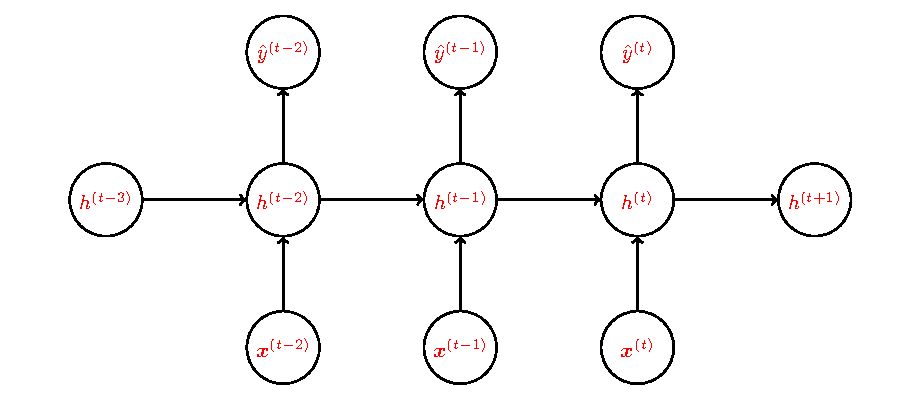
\includegraphics[scale=0.75]{01-unrolled_rnn}
\end{figure}

\newpage 

\noindent \textbf{Answer (continued):} \\

\noindent Now for the gradient calculations, let $\sigma'(\bm{f}_{1}^{(t-1)}) = \frac{\partial \bm{h}^{(t-1)}}{\partial \bm{f}_{1}^{(t-1)}} = diag\left(\bm{h}^{(t-1)} \circ (1 - \bm{h}^{(t-1)}) \right)$.%
%
\footnote{This definition was also with some assistance from the solution set. Once this is set the derivations follow naturally from the previous solutions.} %
%
\newline 
First, $\frac{\partial J ^{(t)}}{\partial \bm{L}_{x^{(t-1)}}}$:
%
\begin{align}
	\frac{\partial J ^{(t)}}{\partial \bm{L}_{x^{(t-1)}}} &= %
		\frac{\partial J ^{(t)}}{\partial \bm{h}^{(t-1)}} %
		\frac{\partial \bm{h}^{(t-1)}}{\partial \bm{f}_{1}^{(t-1)}} %
		\frac{\partial \bm{f}_{1}^{(t-1)}}{\partial \bm{L}_{x^{(t-1)}}} \nonumber \\
	%
		&= \bm{\delta}^{(t-1)} \sigma'(\bm{f}_{1}^{(t-1)}) \bm{I}^{T} \nonumber 
\end{align}
%
\hskip1em

\noindent Now with respect to $\bm{I}$ at the previous time point:
%
\begin{align}
	\frac{\partial J ^{(t)}}{\partial \bm{I}} &= %
		\frac{\partial J ^{(t)}}{\partial \bm{h}^{(t-1)}} %
		\frac{\partial \bm{h}^{(t-1)}}{\partial \bm{f}_{1}^{(t-1)}} %
		\frac{\partial \bm{f}_{1}^{(t-1)}}{\partial \bm{I}} \nonumber \\
	%		
		&=  (\bm{e}^{(t-1)})^{T} \bm{\delta}_{1}^{(t-1)} \sigma'(\bm{f}_{1}^{(t-1)}) \nonumber
\end{align}
% 
\hskip1em

\noindent And finally, with respect to $\bm{H}$ at the previous time point:
%
\begin{align}
	\frac{\partial J ^{(t)}}{\partial \bm{H}} &= %
		\frac{\partial J ^{(t)}}{\partial \bm{h}^{(t-1)}} %
		\frac{\partial \bm{h}^{(t-1)}}{\partial \bm{f}_{1}^{(t-1)}} %
		\frac{\partial \bm{f}_{1}^{(t-1)}}{\partial \bm{H}} \nonumber \\
	%
		&= (\bm{h}^{(t-2)})^{T} \bm{\delta}^{(t-1)} \sigma'(\bm{f}_{1}^{(t-1)}) \nonumber
\end{align}

\vskip2em

%\newpage
%----------------------
\subproblem{d}{Computational Complexity (4 pts)}
\textit{Given $\bm{h}^{(t-1)}$, how many operations are required to perform one step of forward propagation to compute $J^{(t)}(\theta)$? How about backpropagation for a single step in time? For $\tau$ steps in time? Express your answer in big-O notation in terms of the dimensions $d$, $D_{h}$, and $|V|$. What is the slow step?}
%


\vskip2em

\noindent \textbf{Answer:} \\

\noindent For forward propagation, there are 3 transformations that will impact run time and we can express the complexity as a function of the dimensions of those transformations. These are: 1) the input word representation matrix ($\bm{I}$); 2) the hidden transformation matrix ($\bm{H}$); and 3) the output word representation matrix ($\bm{U}$). In big-O notation:
%
\begin{align}
	\text{Forward-prop} &= O\left( (d \times D_{h}) + D_{h}^{2} + (D_{h} \times |V|) \right) \nonumber
\end{align}
%
\vskip1em

\noindent And for backward propagation, it's largely the same thing; however, we need to take the number of time steps, $\tau$, that we're propagating errors to:
%
\begin{align}
	\text{Backward-prop} &= O\left( (d \times D_{h}) + D_{h}^{2} + \tau (D_{h} \times |V|) \right) \nonumber
\end{align}
%
\vskip1em

\noindent Finally, the slow part is the last step when we are taking the softmax of the output word matrix. This is slow because we need to construct a proper probability distribution over the whole of $|V|$, which can be extremely large: i.e., the $O(D_{h} \times |V|)$ piece from $\bm{U}$.


\end{document}
